\documentclass[letterpaper,11pt,twocolumn]{article}
\usepackage{usenix,graphicx,times}

%\usepackage{graphics, graphicx, fancyhdr, epsfig, amstext}
%\usepackage{amsmath, amssymb, xspace, setspace, times, color}

\usepackage{graphicx}
\graphicspath{}

\usepackage{hyperref}

\usepackage{listings}
\usepackage{xcolor}
% style for code listings (from overleaf)
\definecolor{codegreen}{rgb}{0,0.6,0}
\definecolor{codegray}{rgb}{0.5,0.5,0.5}
\definecolor{codepurple}{rgb}{0.58,0,0.82}
\definecolor{backcolour}{rgb}{0.95,0.95,0.92}
\lstdefinestyle{mystyle}{
    backgroundcolor=\color{backcolour},
    commentstyle=\color{codegreen},
    keywordstyle=\color{magenta},
    numberstyle=\tiny\color{codegray},
    stringstyle=\color{codepurple},
    basicstyle=\ttfamily\footnotesize,
    breakatwhitespace=false,
    breaklines=true,
    captionpos=b,
    keepspaces=true,
    numbers=left,
    numbersep=5pt,
    showspaces=false,
    showstringspaces=false,
    showtabs=false,
    tabsize=2
}
\lstset{style=mystyle}

\usepackage[
  backend=biber,
  style=alphabetic,
]{biblatex}
\addbibresource{citations.bib} %Imports bibliography file

\usepackage{stfloats}
\usepackage{float}

\usepackage{lipsum}

% \usepackage{todonotes}

\begin{document}

\title{A fast and memory-safe asynchronous gRPC bookstore server (and clients)}
\date{Feb 23, 2023}

\author{
  {\rm Ye Shu}\\
       Williams College\\
       ys5@williams.edu
\and
  {\rm Jason Lee}\\
       Williams College\\
       jml8@williams.edu
}

\maketitle

\thispagestyle{empty}
%\pagestyle{empty}

% \begin{abstract}
% Abstract is optional.
% \end{abstract}

\section{Introduction}

With a growing interest in Distributed Systems nowadays, the demand to run programs, call functions, and pass in and out data across systems distributed across network has also increased.
While many of the modern software pieces implement this by using RESTful APIs, RPC (Remote Procedure Calls) have also gained traction. Unlike RESTful APIs that must be stateless and are designed around resources, RPCs are designed around actions. Hence, RPCs remain popular for their flexibility.

In our submission, we create a gRPC server and multiple clients in various languages. 
We specifically chose gRPC since it is one of the most prevalent RPC libraries now in industry and also because it is the RPC library with best performance (due to the tight serialization packing and the default HTTP/2 usage).
Eventually, our server is able to handle buy requests with \textbf{0.263ms} and search requests with \textbf{0.107ms} concurrently.
Moreover, we have written our server with high availability and reliability. More importantly, the server is guaranteed to be memory and concurrency safe by its design, which we shall get into later in this paper.

The paper is laid out in the following way: Section 2 lays out the overview for the architecture, describing how our clients and servers communicate with each other, and what roles they have served. Section 3 goes into the implementation details, discussing the various design choices we made along the way, and the trade offs we have made. Section 4 presents some empirical evaluation metric for the server to present its strength. Last but not least, Section 5 concludes our write-up and discusses potential for future work.

\section{Architectural Overview}

We built our server in Rust \cite{rust}, utilizing gRPC \cite{grpc}'s specific interface description language protobuf \cite{protobuf}. After defining the interface in our .proto file, gRPC could then compile a pair of stubs (one for packing and unpacking parameters in a procedure call and the second to form the connection between client and server). The design of the stubs is symmetrical from client to server and server to client. The difference lies in the information sent; the client sends requests and the server sends back replies. 

\begin{figure}[htb]
    \centering
    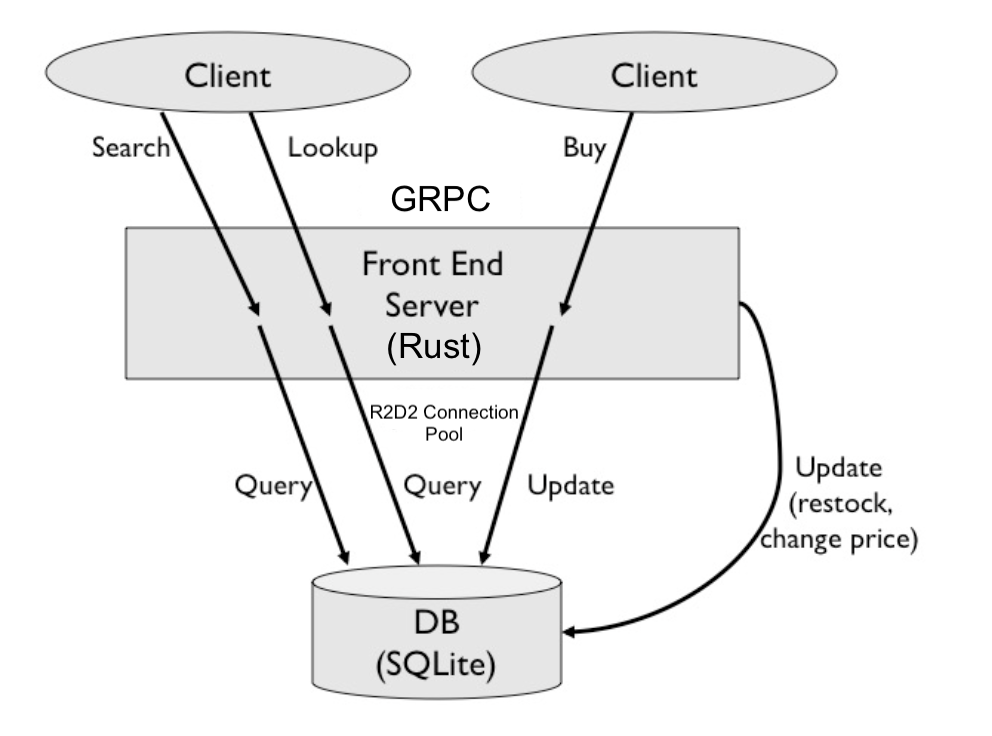
\includegraphics[width=\linewidth]{diagram.png}
    \caption{Overall architecture of communication between the Server, Client, and database.}
    \label{fig:architecture}
\end{figure}

The client or server calls the protobuf through a local procedure call containing the parameters for the remote procedure. The protobuf stub then marshals (stores parameters) from the local procedure call into a message. This message is then handled by the gRPC for transmission. The protobuf-marshaled message is unmarshaled and marshaled by the gRPC, which handles creating the HTTP connection between client and server. It attaches the appropriate headers and sends this new message to the recipient end's gRPC stub. The recipient gRPC stub unmarshals the message which is then handled by the recipient's protobuf stub. The protobuf stub marshals the message and then unmarshals it finally, processable by the recipient. 

If the recipient is the client, our bookstore simply printed out the results of the function call. On the other hand, a valid message to the server would likely require a query and perhaps an update of the database, which is stored on a local file in the server. To handle the connection between our Rust server and the SQLite database, we used the rusqlite crate. Our solution for dealing with high traffic conditions was a connection pool, using the r2d2-sqlite crate. Instead of opening a new database connection for each client, an inefficient operation that can be limiting in high traffic scenarios, the connection pool stores a recyclable set of open connections. These connections are handed out on a need basis and returned once the job is fulfilled. With this connection, the server can either serve the client, fulfilling its procedure calls, or it can perform its own commands to access or update the server such as restocking. For a full list of commands available to client, server, and both refer to Table \ref{tab:commands}.

\begin{table*}[bt]
\centering
 \begin{tabular}{||l l l l||} 
 \hline
  & Command & Usage & Description \\ [0.5ex] 
 \hline
 \hline
 Client & ping & \texttt{ping} & Tests connection to server \\ 
  & search & \texttt{search <topic>} & Search for books by topic \\ 
  & lookup & \texttt{lookup <id>} & Lookup book information by id \\ 
  & buy & \texttt{buy <id>} & Buy book given id \\ [0.5ex]
\hline
Server & list & \texttt{list} & List all books in DB \\
  & restock & \texttt{restock [amount]} & Restock all books up to [amount]. Default is 20. \\
  & update & \texttt{update <id> <price>} & Update price of a book \\
  & log & \texttt{log} & Print out recent transactions \\ [0.5ex]
\hline
Both  & help & \texttt{help} & Prints a help message regarding command usage \\
 & exit & \texttt{exit} & Exits the program \\ [0.5ex] 
 \hline
 \end{tabular}
 \caption{List of supported commands on clients and servers.}
 \label{tab:commands}
\end{table*}

\section{Implementation Details}

% \subsection{Choice of Language and Tech Stack}
% why rust? memory safe
% \todo[inline]{Might delete this section}

\subsection{Server Concurrency with Async Green Threads}
One thing that makes implementation of our server hard is that the server must simultaneously support a commandline like interface for users to lookup and change values in the database.
To realize this feature, we have to run the gRPC server and the commandline utility concurrently.
In the past lab, we had already experienced operating system threads and learned how inefficient they might be (since the OS scheduler usually polls all threads, even though most of the threads aren't even active). Thus, we will continue using the event-driven approach. However, this time we shall implement the event-driven approach differently, with asynchronous runtime.

In our design, we have made use of tokio \cite{tokio}, an asynchronous runtime in Rust. If you are unfamiliar with Rust and Tokio, just think about Node, which is an asynchronous event-driven runtime environment in JavaScript.
In spawning threads inside tokio runtime, we create asynchronous green threads (as opposed to OS threads) that offers concurrency but not parallelism.
Therefore, since we are always running in one OS thread and have a runtime system to handle the scheduling of green threads, we would have better performance when compared to the OS scheduler (since we would also have more information available to us, e.g. if the stdin reader has become available). 

Moreover, given the async nature of both threads, we have to implement them asynchronously as well. Thus, we have used an asynchronous gRPC implementation named tonic \cite{tonic} and implemented an asynchronous commandline ourselves. 

Then, all our rpc handler code must also be written asynchronously as well. This used to be a pain in JavaScript with all the callback functions and how they capture, consume, or access variables. Luckily, with Rust we are able to handle everything easily, with locking mechanisms and atomic reference counters. In our implementation, we used a thread-safe database connection pool to share connections to databases safely while avoiding both concurrency issues and the overhead of creating and tearing multiple database connections. 

Regarding the implementation of async commandline, the code is quite similar to a synchronous ones, except that we call on an asynchronous function \texttt{buf\_reader.next\_line().await} to read results from a buffered reader. Note that here we explicitly use the \texttt{await} keyword to wait for the \texttt{Future} to be fulfilled (in other words, we block the thread until stdin has become available to read). This makes the async function synchronous-like in behavior (but is still scheduled asynchronously by the runtime to achieve performance).

\subsection{Concurrency and Data Sharing}

A pain with concurrent programming is to handle the data that must be shared across threads.
Traditionally, most programming languages only provide mutex (mutual exclusion) locking mechanisms. 
Hence, for a thread1 to access some shared memory area $m$, it must acquire a lock first. Note that the lock acquisition action must be atomic, and thus extremely slow.
In some modern languages, an alternative approach called message passing (e.g. the \texttt{channel}'s in Go and Rust) have also gained popularity. The channels are completely lock free, since they are unidirectional data structures that allows one (or multiple) thread acting as data producer to send things to another thread acting as data consumer (which is the most common data sharing scenario).

In our project, we have used both methods to share data across gRPC server and commandline threads. We have used message passing to pass the shutdown command from commandline when it reads in an \texttt{exit} command from user to the server for graceful shutdown. On the other hand, the database connection pool has to use shared memory (i.e. locking) mechanism, since there exists multiple consumer threads. This a major limitation for message passing, as its lock-free nature dictates that at most one thread can act as the consumer (while infinitely many can be producers that send data into the channel).

For the logging mechanism, we have specifically chosen the memory sharing mechanism, even though we only have one consuming threads. This is because for a channel to work, we must also have a thread that constantly polls the channel to handle the input, which transitions the burden to the programmer to handle yet another type of event. Although it is possible to use mechanisms like \texttt{select}, it is nevertheless painful to implement. 
Therefore, we have traded a slight performance hit for development agility in this case. With that being said, if the lock has exhibited to be a bottleneck, we will always have the opportunity to switch to message passing. 

\subsection{SELECT-UPDATE data races}

Here, we have a classic problem with the sql \texttt{SELECT}-\texttt{UPDATE} query pattern while handling buying requests.
For any incoming buying requests, before we update the table, we must first check if the available count of the book is greater than 1. Then, only if it is greater than 1 can we do the subtraction update, thus selling the book to a user.
The pseudocode will look vaguely like this.
\begin{lstlisting}[language=sql,label=lst:use,caption={Psudocode for the buy handler.}]
result := sql.exec(`SELECT stock FROM books WHERE id = 53477`);
if (result >= 1) {
    sql.exec(`UPDATE books SET stock = stock - 1 WHERE id = 53477`);
    return "bought successfully";
} else {
    return "sold out";
}
\end{lstlisting}

Now, assume we have two threads who are handling the request from two users at the same time. We shall name them $thread_1$ and $thread_2$. 
The following unfortunate scenario might happen:
\begin{enumerate}
    \setlength{\itemsep}{0pt}
    \setlength{\parskip}{0pt}
    \item $thread_1$ finished execution of line 1, receives the result of 1.
    \item Scheduler pauses execution of $thread_1$, and resumes $thread_2$.
    \item $thread_2$ starts at line 1, receives the same result of 1, and continues to sell the book.
    \item Scheduler discovers that $thread_2$ finishes, and switches back to $thread_1$.
    \item $thread_1$ sees that result is 1, so continues to sell the last copy of the book (although the book has already been sold by $thread_2$).
\end{enumerate}

Naturally, the solution to avoid race conditions is by locks, or mutual exclusion structures. We can use locks to protect the entire code segments listed above (which become ``critical regions'' in this context) so only at most one thread can execute them at one given time.

However, locks are not the best solution to our specific scenario (database read-write) either.
Firstly, locks are extremely costly. The lock data structure must be atomic. In other words, when we acquire a lock, the CPU pipeline must be stalled (which affects all threads) to update the status of the lock to all threads. 
Secondly, locks do not fully solve the problem either. Imagine that we have multiple servers running simultaneously, implementing a lock at the server-level only stops the concurrent access within one server. The problem above could still occur between two servers, if you switch $thread_1$ and $thread_2$ to be $server_1$ and $server_2$.

Therefore, the best solution is to implement the locking mechanism at the database level. In fact, all databases are designed to handle concurrency in its nature, and are most efficient at handling locks. For most databases, such as MySQL and PostgreSQL, the \texttt{SELECT} clause has a specific option called \texttt{SELECT ... FOR UPDATE} \cite{mysql}\cite{postgres} that locks the retrieved rows for write. This mechanism ensures that the retrieved rows are always up to date and cannot be modified by other connections to the database before the current transaction is committed (i.e. when the write lock is released by the current connection).

Unfortunately, SQLite does not support the \texttt{SELECT ... FOR UPDATE} behavior. However, we can still manually acquire a write lock that achieves the same effect. To do so, we must use \texttt{BEGIN IMMEDIATE} (instead of \texttt{BEGIN}, which uses deferred mode \cite{sqlite}) to start a transaction, which acquires the write lock immediately.
Therefore, since we must acquire a write lock at the beginning of each buy transactions, we ensure that only one connection can handle the relevant data at the same time, thus solving the data race issue.

% the problem with select-update pattern and concurrency
% solution: locks
% BUT: we don't implement locks at program level

% SELECT ... FOR UPDATE
% % https://dev.mysql.com/doc/refman/8.0/en/innodb-locking-reads.html
% % https://www.postgresql.org/docs/current/sql-select.html

% write lock (with BEGIN IMMEDIATE)

% \subsection{SQLite isolation modes}

% \todo[inline]{only if we had time left}
% connection pools

% our solution: database locking mechanism
% three types of sqlite isolation modes

% If we have time: the excessive error handling in Rust (with Outcome and Result)

\section{Evaluation}

\subsection{Experiment Setup}

To evaluate the performance of our server, we ran multiple requests sequentially as well as concurrently, and measure their finished time to determine the capacity of our server.

Among all operations, we have chosen two to measure, the \texttt{search} operation and the \texttt{buy} operation. The search operation corresponds to a readonly database transaction, while the buy operations corresponds to a write database transaction (even if we never updated the database due to out of stock, we still acquired a write lock).

The evaluation code is written in Rust, for its simplicity of thread operations. For the sequential evaluation, we create one gRPC client, and sequentially executes 5,000 operations. We have selected 5,000 instead of 500 as instructed by the course project requirement, since 500 requests can be done within a second, and may not offer precise approximations of the average time taken.
For the concurrent evaluation, we spawn multiple threads, and then within each thread creating one gRPC client to execute $$\frac{\textnormal{total request}}{\textnormal{num of client}}$$ number of requests.

The experiment code are ran on an 2020 M1 MacBook Air, with both the server and client running on the same machine, communicating using loopback network interface to minimize the effect of network latency. Prior to each experiment, the stock of the books are restocked to 1,000. Hence, For the buy request experiments, we should receive 1,000 successes and 4,000 out of stock responses. When we run the clients concurrently, the experiment also empirically checks our server for thread-safety.

Both the source code and the raw data (detailing the end time of each request and the returned response result) for the evaluation is committed in our repo. The source code can be found at \texttt{/server/src/eval.rs} and the raw data can be found as \texttt{.csv} forms under \texttt{/server} directory.

\subsection{Results}

We will present our results section to answer each of the following research questions (RQ). Some of them will be accompanied by figures to easily illustrate the result.

\textbf{RQ1: How does our server perform when handling requests sequentially?}

For 5,000 sequential buy requests, our experiment started at \texttt{16:05:38.087558} and finishes at \texttt{16:05:40.412229}, which takes \texttt{2.324671} seconds. On average, each request took \textbf{0.46493 ms}, including the thread setup time.
With our experimental setup, 1,000 of the buy requests succeed, which is expected as we only made 1,000 stocks of the book available.

% sequential buy
% \begin{verbatim}
% time start: 2023-03-14 16:05:38.087558 -04:00
% time end: 2023-03-14 16:05:40.412229 -04:00
% time diff: 2.324671s
% num success: 1000
% \end{verbatim}

For 5,000 sequential search requests, our experiment started at \texttt{16:12:04.642339} and finishes at \texttt{16:12:07.138586}, which takes \texttt{2.496247} seconds. On average, each request took \textbf{0.49925 ms}, including the thread setup time.

It is surprising to discover that the sequential search requests took slightly longer time than buy requests. We conjecture that sequential requests took longer because their return type is much more complicated. In addition to the boolean success value and a message, which the buy request also returns, the search requests also return the complete information of two books (id, title, topic, stock, price) in the form of vectors. It's possible that the marshaling and marshaling of the struct vectors slow down the search requests.

% sequential search
% \begin{verbatim}
% time start: 2023-03-14 16:12:04.642339 -04:00
% time end: 2023-03-14 16:12:07.138586 -04:00
% time diff: 2.496247s
% num success: 5000
% \end{verbatim}

\textbf{RQ2: How does our server perform when handling requests concurrently?}

To evaluate concurrent requests, we ran two experiments, executing 5,000 buy requests with 10 clients and with 100 clients. Similar to other experimental setups, we initialize the books to have 1,000 stocks and observe how many of the buy requests succeed.

In the first experiment with 10 clients, all requests are finished within \texttt{1.316011} seconds. Thus, on average each request takes \textbf{0.26320 ms}.
In the second experiment with 100 clients, all requests are finished within \texttt{1.297990} seconds. Thus, on average each request takes \textbf{0.25960 ms}.

\begin{figure}[thb]
    \centering
    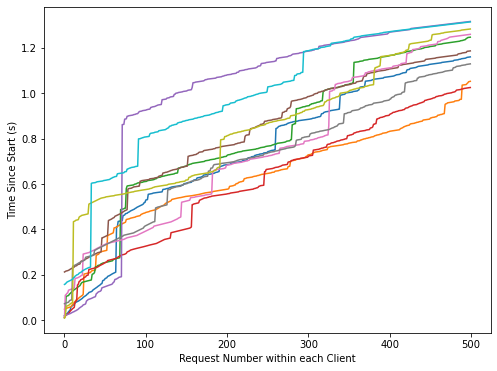
\includegraphics[width=\linewidth]{time_buy_10.png}
    \caption{The finish time of each request in ten concurrent clients}
    \label{fig:time-buy-10}
\end{figure}


Furthermore, we have measured the finish time of each individual requests in each clients, and have plotted them for the first experiment in Figure \ref{fig:time-buy-10}. It is evident that the first 50 requests are the most time-consuming, and the time taken by following requests are much shorter (as seen by the flatter curve). However, we do not currently have a good explanation for this observation. Our best guess is that the initial phase is more complicated, and the schduler performs worse than the later phase. This is evident by some threads getting blocked much longer than others (as seen by the vertical lines in the figure).

When compared to the 0.46493ms in the sequential buy requests, it is apparent that time is significantly improved by 10 concurrent clients. 
However, with more concurrent clients (10 to 100), the request processing time is not significantly reduced. 
We conjecture that with more concurrent clients, the overhead of creating clients and scheduling different threads will start to dominate the time taken. Therefore, when we increase the number of clients, we face a reduced marginal benefit. Eventually, we might even get higher average time with increased number of clients. We shall elaborate more on this in our discussion of RQ4.

% buy-10 client
% \begin{verbatim}
% time start: 2023-03-14 16:17:48.313266 -04:00
% time end: 2023-03-14 16:17:49.629277 -04:00
% time diff: 1.316011s
% num success: 1000
% \end{verbatim}

% buy-100-client
% \begin{verbatim}
% time start: 2023-03-14 16:18:29.548516 -04:00
% time end: 2023-03-14 16:18:30.846506 -04:00
% time diff: 1.297990s
% num success: 1000
% \end{verbatim}

\textbf{RQ3: Does the type of request matter?}
Yes and no. For sequential 5,000 requests, the average time for buy and search requests are quite similar. Further, the average time for search (0.49925ms) is slightly higher than that for buy (0.46493ms). We think it might be related to the marshaling and unmarshaling of complicated struct vector data.

However, for the concurrent connections, search becomes much faster than buy requests. We ran experiments of 5,000 requests with 10 concurrent clients for both buy and search requests. Search only took \texttt{0.535931}s, whereas buy took \texttt{1.316011}s. On average, each search requests took \textbf{0.10719ms} whereas each buy requests took \textbf{0.26320ms}. For a better comparison, you can also refer to RQ4 and Figure \ref{fig:time-concurrent}.

The huge difference is, however, explainable. For search requests, they return a more complicated data structure and the database transaction is read-only. Thus, the operation can be done without any lock structures. However, the buy requests must acquire a write lock of the database. Therefore, the database can serve at most one buy request at a given time. This mutual exclusion guarantees the thread-safety of the write operation but at the same time reduces the throughput and thus benefit of concurrency.

\textbf{RQ4: How much performance gain does concurrency provides?}
In this experiment, we ran the same evaluation code on both operations for 5,000 times, with number of concurrent clients ranging from 1 to 20.
The average request time against the number of concurrent clients for both the lock-free operation search and the locked opeartion buy are plotted in Figure \ref{fig:time-concurrent}. 

We expected the performance gain to be very significant with the addition of the first few threads, which turns out to be correct. Moreover, the performance gain for buy becomes very insignificant just past the third client. This is understandable due to the locking mechanism.
To our surprise, the performance gain for the lock-free search operation is pretty insignificant as well. The gain from 3 concurrent client to 10 is just 1.20 to 0.85s. And the time sees no improvement further than 10 clients.

\begin{figure}[tbh]
    \centering
    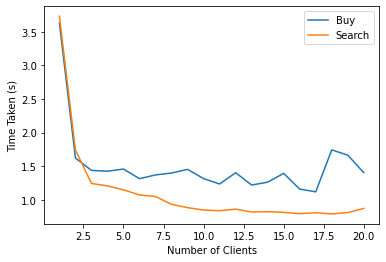
\includegraphics[width=\linewidth]{time_concurrent.png}
    \caption{For search, the time taken decreases sharply at first but quickly evens out at around 10 clients. For buy, no significant improvement can be seen after 3 clients.}
    \label{fig:time-concurrent}
\end{figure}

The result confirms our previous hypothesis that concurrency is very beneficial at first, but faces sharp decreasing marginal utility. However, we did not expect the marginal utility to decrease to almost zero at the small number of 10 clients.

\section{Conclusion \& Discussions}

To conclude, we have presented a highly performant, reliable, memory-safe, and thread-safe gRPC server and its clients in this paper. We have demonstrated that our server can handle lock-free read-only database requests within 0.10719ms and locked read-write requests within 0.26320ms on average.
Furthermore, we have made multiple observations regarding the concurrency performances. It seems that most of the concurrent requests have started to take longer, but as the concurrent threads continue execution, the average time becomes lower. Moreover, some threads seem to be blocked for as long as 0.4 seconds at first, whereas none of the threads are blocked so long later on.
In addition, we have also discovered that it is less economical to send out locked requests with more than 2 concurrent connections. On the other hand, for lock-free requests, adding concurrent connections provides improvements, but gradually decreases over time and provides no benefit at all when beyond a certain point.

We have certainly enjoyed the process of writing this project. We feel that Rust is a unique and fun language to write. It has very robust error handling with \texttt{Result} and \texttt{Option} wrappers, and we can chain their operations almost monadically. Rust has also borrowed many features from functional programming languages, including mapping over iterators and using closures. 

Furthermore, although the borrow checker has created much trouble for us to explicitly say which arguments are borrowed and which are moved, they nevertheless provide guarantee for memory safety (especially the memory safety across threads), which is a trade off well worth it in our humble opinions. One last thing to comment on, the Tokio runtime system really makes asynchronous event-driven architecture easy to write with a robust and performant language. I almost felt like writing Node.JS code but with much more confidence that my code is going to run correctly with type guarantees and lifetime guarantees.


\medskip
\nocite{*}
\printbibliography

%\bibliographystyle{plain}
%\bibliography{bibfile}

\end{document}
